\chapter[Diagramas]{Diagramas}

 \subsection{Banco de Dados}

  \begin{figure}[!htb]
        \centering
        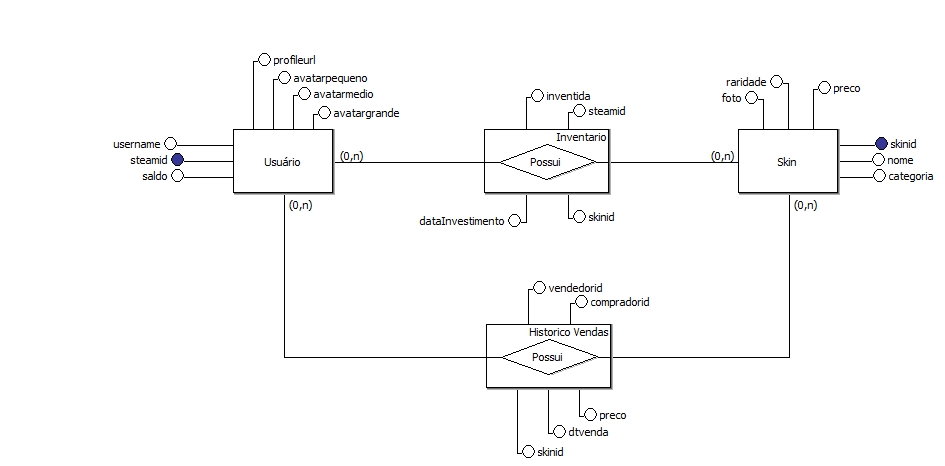
\includegraphics[scale=0.5]{Imagens/Relacionamento.png}
        \caption{Modelo Entidade Relacionamento - Banco de Dados}
 \end{figure}

  \begin{figure}[!htb]
        \centering
        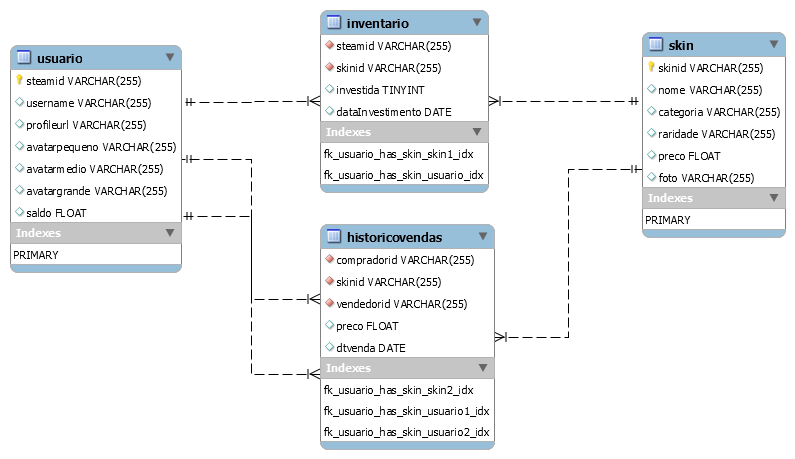
\includegraphics[scale=0.6]{Imagens/Logico.png}
        \caption{Modelo Lógico - Banco de Dados}
 \end{figure}

  \begin{figure}[!htb]
 \subsection{Casos de uso}
        \centering
        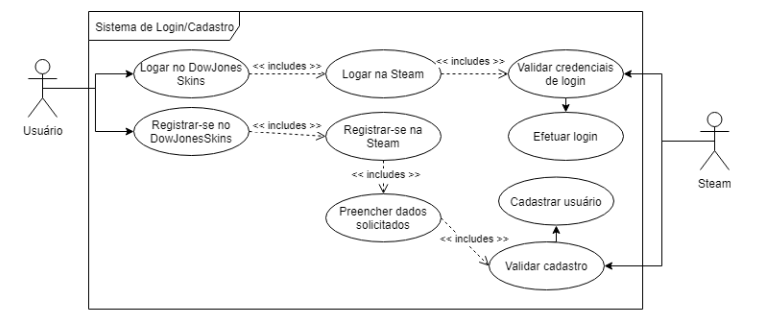
\includegraphics[scale=0.6]{Imagens/login.png}
        \caption{Login do usuário}
 \end{figure}

  \begin{figure}[!htb]
        \centering
        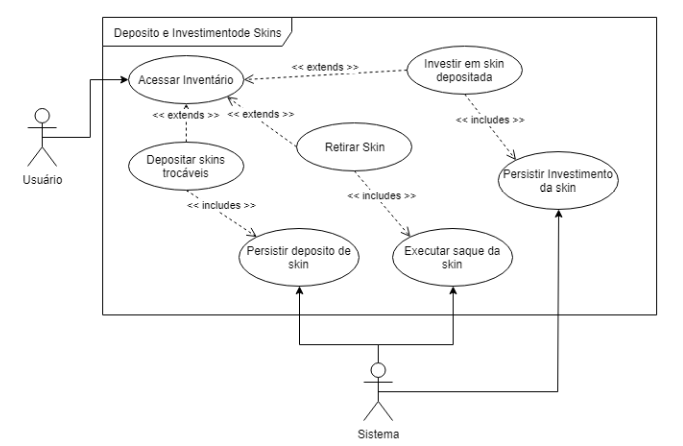
\includegraphics[scale=0.6]{Imagens/deposito.png}
        \caption{Depósito de Skins}
 \end{figure}

  \begin{figure}[!htb]
        \centering
        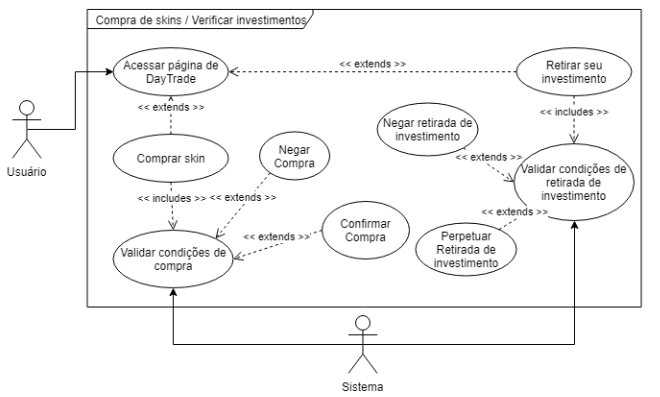
\includegraphics[scale=0.6]{Imagens/compra.png}
        \caption{Compra de Skins}
 \end{figure}

  \begin{figure}[!htb]
        \centering
        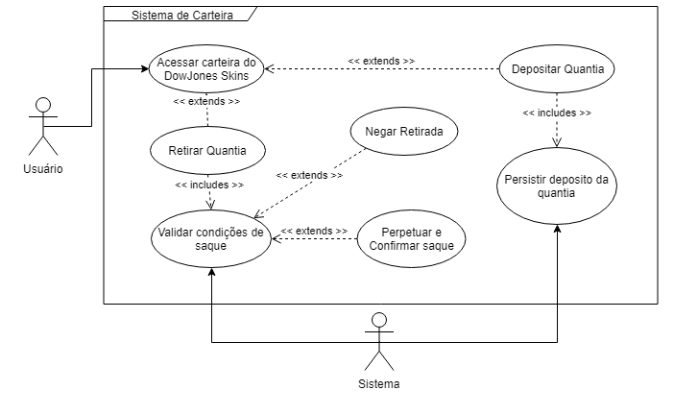
\includegraphics[scale=0.6]{Imagens/carteira.png}
        \caption{Carteira do usuário}
 \end{figure}